\documentclass{beamer}

\usepackage[beamer]{shortcut}
\graphicspath{{./images/}}

\def\biblio{
    \nobibliography{../../library}
    \def\biblio{}
}

\institute{INRIA Saclay}
\author{Thomas Moreau}
\title{
    Working group: HPC and IA
}

\setbeamertemplate{title page}[frame]
\def\extraLogo{
    \url{https://tinyurl.com/numpex-ia}
}

\begin{document}

    \begin{frame}
        \titlepage
        % \biblio{}
    \end{frame}

    \begin{frame}{IA - Applications}
        \begin{columns}[T]
            \column{.5\textwidth}
            \centering
            {\bf Tabular data}\\[3em]
            \includegraphics[width=.4\textwidth]{logo_database.png}\\
            {\bf Database}\\[1em]
            \begin{itemize}
                \item Structured data,
                \item Reasonable scale.
            \end{itemize}
            \column{.5\textwidth}
            \centering
            {\bf Complex data}\\[.5em]
            \includegraphics[width=.3\textwidth]{logo_chatgpt}
            
\includegraphics[width=.3\textwidth]{logo_copilot}
            
\includegraphics[width=.3\textwidth]{logo_midjourney}\\[1em]
            {\bf Text \hskip4ex Code\hskip 4ex Images }\\
            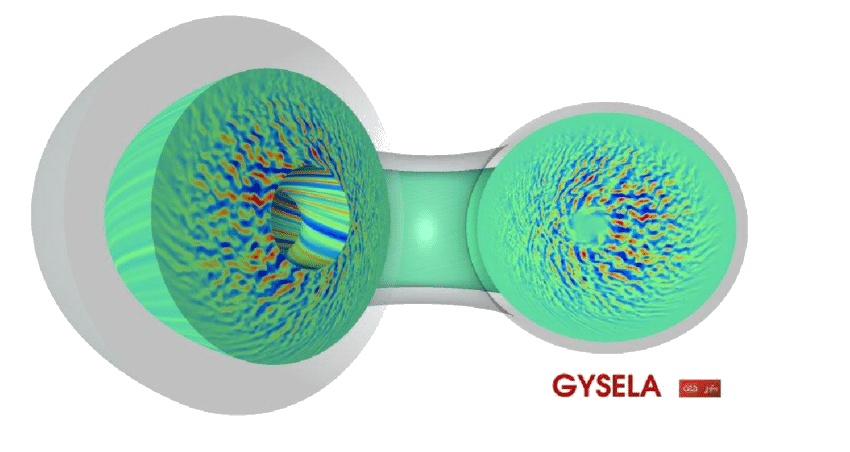
\includegraphics[width=.45\textwidth]{gysela}
            
\includegraphics[width=.45\textwidth]{logo_skao}\\[1em]
            {\bf ML for physical sciences}\\[1em]
            \begin{itemize}
                \item Unstructured data,
                \item Huge scale.
            \end{itemize}
        \end{columns}
    \end{frame}

    \begin{frame}{IA - scales}
        \begin{columns}[T]
            \column{.5\textwidth}
            \centering
            {\bf Tabular data}\\[1em]
            \includegraphics[width=.4\textwidth]{logo_database.png}\\
            {\bf Database}\\[1em]
            \begin{itemize}
                \item Large number of rows\\($n$ samples),
                \item Small to medium number of columns ($p$ features).
            \end{itemize}
            \column{.5\textwidth}
            \centering
            {\bf Complex data}\\[3em]
            {\bf Text \hskip4ex Code\hskip 4ex Images }\\[1em]
            {\bf ML for physical sciences}\\[3em]
            \begin{itemize}
                \item Very to Huge scale.
                \item Sometime many samples, sometime not.
            \end{itemize}
            \strongpoint{Very heterogeneous}
        \end{columns}
    \end{frame}

    \begin{frame}[t]{IA - tools}
        \begin{columns}[T]
            \column{.5\textwidth}
            \centering
            {\bf Tabular data}\\[3em]
            % \includegraphics[width=.3\textwidth]{logo_numpy}
            \includegraphics[width=.4\textwidth]{logo_pandas}
            \includegraphics[width=.4\textwidth]{logo_sklearn}\\[2.5em]
            \begin{itemize}
                \item Stable stack,
                \item Development: interoperatiblity, nested parallelism, \dots
            \end{itemize}
            \column{.5\textwidth}
            \centering
            {\bf Complex input data}\\[2em]
            \includegraphics[width=.4\textwidth]{logo_pytorch}
            \includegraphics[width=.4\textwidth]{logo_jax}\\[1em]
            \begin{itemize}
                \item Moving stack
                \item Support various hardware
                \item autodiff, jitting, \dots
            \end{itemize}
        \end{columns}
        \vskip1em

        {Most of the stack in Python, with a strong focus on user-friendly tools.}
    \end{frame}

    \frame{
        \frametitle{Subjects}

        \begin{itemize}\itemsep2em
            \item What are the task we are interested in? How to define them in a way that is understandable by the 2 communities?
            \item Where to plug in IA? How to allow the 2 communities to interact?
            \item Which tools and how to impact them? How to have interoperatiblity?
            \item Is there a need for specific algorithms (online/distributed learning or inference) due to the data scale? Specific architectures with NAS?
            \item How to impact IA? (LLM/Bloom?)
        \end{itemize}
    }

    \frame{
        \frametitle{What to do?}


        \begin{itemize}\itemsep2em
            \item How to leverage Physic informed machine learning? (PINN, NeuralODE, ) for surrogate models? for anomaly detection, ?
            \item How to leverage the Graph Neural Networks?
            \item Compression, multi-resolution, super resolution?
            \item Event detection: in signals, in logs, \dots
        \end{itemize}
    }

    \frame{
        \frametitle{Physic Informed ML}

        \centering
        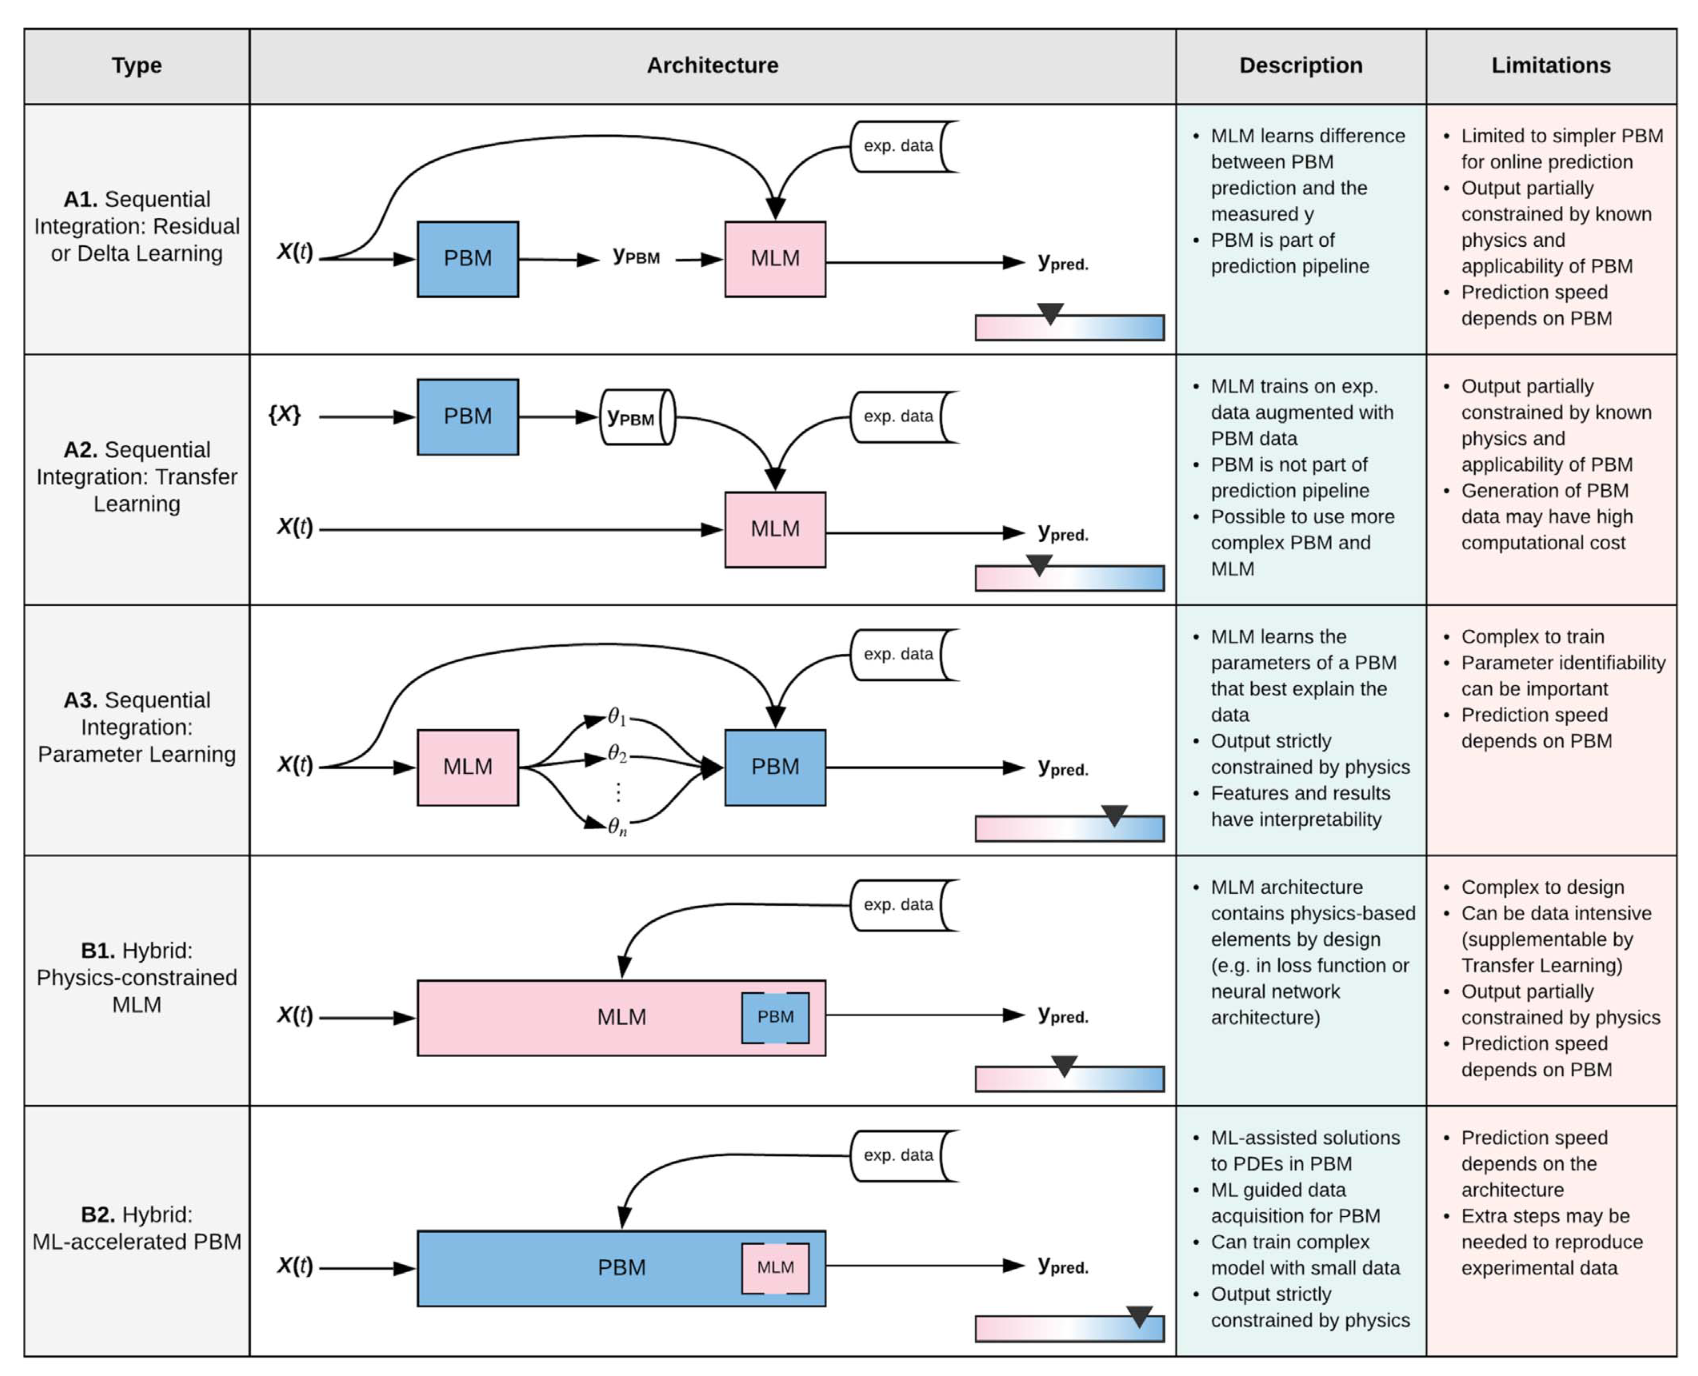
\includegraphics[width=.8\textwidth]{physic_informed_ml}\\
    }

\end{document}